\section{Auswertung}

\subsection{Statistische Methode}

\subsubsection{Temperaturverläufe}

Zuerst wurden in einer Messung die Temperaturen der, der Heizquelle, ferenen Thermoelemente gemessen. Dabei liegt T1 am breiteren der beiden Messingprobenstäbe und T4 am schmaleren. T5 liegt am Aluminium Stab und T8 am Edelstahlstab. Die Temperaturverläufe der einzelnen Messpunkte sehen dabei wie folgt aus:

\begin{figure}[H]
    \centering
    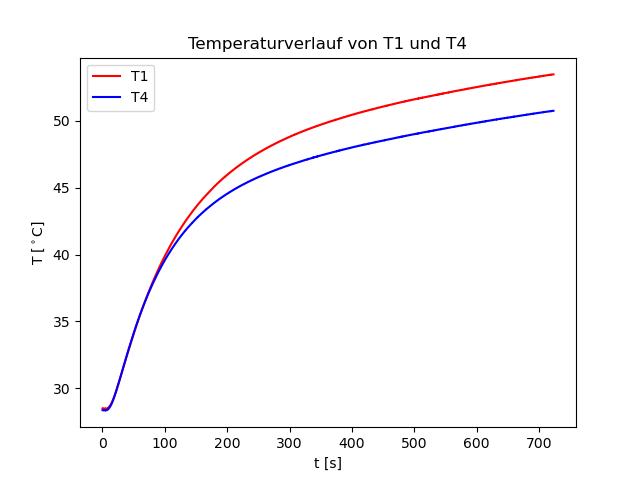
\includegraphics{1.png}
\end{figure}

\begin{figure}[H]
    \centering
    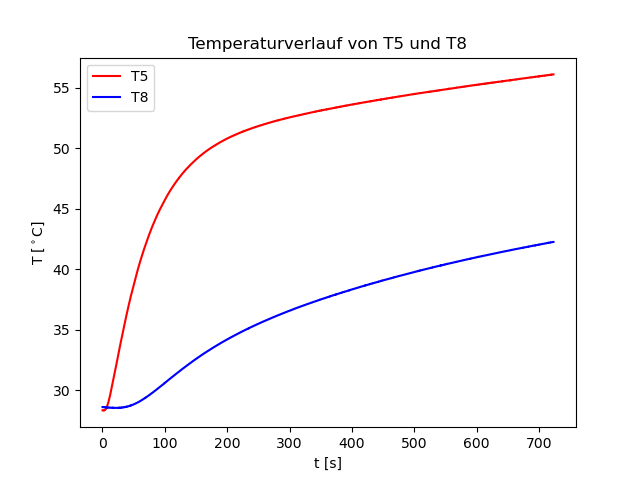
\includegraphics{2.png}
\end{figure}

\subsubsection{Temperatur nach t=700s}

700s entsprechen bei einer Abtastrate von 5 Werten pro Sekunde den Werten in der 3500. Zeile der Tabelle ?. Diese sind allerdings auch noch einemla hier aufgelistet:
\begin{align*}
    T1 = 53.3 ^\circ C  \\
    T4 = 50.59 ^\circ C \\
    T5 = 55.95 ^\circ C \\
    T8 = 42.03 ^\circ C 
\end{align*}

\subsubsection{Wärmestrom $\frac{\Delta Q}{\Delta t}$}

Anschließend soll für 5 verschiedene Meßzeiten der Wärmestrom $\frac{\Delta Q}{\Delta t}$ bestimmt werden. Dazu wird folgende Gleichung verwendet. 
\begin{displaymath}
    \frac{\Delta Q}{\Delta t} = - \kappa A \frac{\partial T}{\partial x}
\end{displaymath}

Dabei ergeben sich für den Wärmestrom folgende Werte: 
\begin{minipage}{\linewidth}
    \begin{table}[H]
        \centering
    \captionof{table}{Berechnete Wärmeströme für t=140s}
    \begin{tabular}{lll}
        \toprule
        Meßzeit [s] & $\frac{\partial T}{\partial x}$ & Wärmestrom  \\
        \midrule
        Messing (breit) & 5.03 & -289.728 \\
        Messing (schmal) & 6.31 & -212.016 \\
        Aluminium & 3.03 & -290.880 \\
        Edelstahl & 13.63 & -256.512 \\
        \bottomrule   
    \end{tabular}
    
    \label{tab:1}
\end{table}
\end{minipage}

\begin{minipage}{\linewidth}
    \begin{table}[H]
        \centering
    \captionof{table}{Berechnete Wärmeströme für t=280s}
    \begin{tabular}{lll}
        \toprule
        Meßzeit [s] & $\frac{\partial T}{\partial x}$ & Wärmestrom  \\
        \midrule
        Messing (breit) & 3.11 & -179.136 \\
        Messing (schmal) & 4.51 & -151.536 \\
        Aluminium & 1.94 & -186.240 \\
        Edelstahl & 11.93 & -229.056 \\
        \bottomrule   
    \end{tabular}
    
    \label{tab:2}
\end{table}
\end{minipage}

\begin{minipage}{\linewidth}
    \begin{table}[H]
        \centering
    \captionof{table}{Berechnete Wärmeströme für t=420s}
    \begin{tabular}{lll}
        \toprule
        Meßzeit [s] & $\frac{\partial T}{\partial x}$ & Wärmestrom  \\
        \midrule
        Messing (breit) & 2.56 & -147.456 \\
        Messing (schmal) & 4.05 & -136,080 \\
        Aluminium & 1.71 & -164.160 \\
        Edelstahl & 10.86 & -208.512 \\
        \bottomrule   
    \end{tabular}
    
    \label{tab:3}
\end{table}
\end{minipage}

\begin{minipage}{\linewidth}
    \begin{table}[H]
        \centering
    \captionof{table}{Berechnete Wärmeströme für t=420s}
    \begin{tabular}{lll}
        \toprule
        Meßzeit [s] & $\frac{\partial T}{\partial x}$ & Wärmestrom  \\
        \midrule
        Messing (breit) & 2.40 & -138.240 \\
        Messing (schmal) & 3.93 & -132.048 \\
        Aluminium & 1.64 & -157.44 \\
        Edelstahl & 10.36 & -198.912 \\
        \bottomrule   
    \end{tabular}
    
    \label{tab:4}
\end{table}
\end{minipage}

\begin{minipage}{\linewidth}
    \begin{table}[H]
        \centering
    \captionof{table}{Berechnete Wärmeströme für t=420s}
    \begin{tabular}{lll}
        \toprule
        Meßzeit [s] & $\frac{\partial T}{\partial x}$ & Wärmestrom  \\
        \midrule
        Messing (breit) & 2.33 & -134.208 \\
        Messing (schmal) & 3.87 & -130.032 \\
        Aluminium & 1.62 & -155.52 \\
        Edelstahl & 10.00 & -192.000 \\
        \bottomrule   
    \end{tabular}
    
    \label{tab:5}
\end{table}
\end{minipage}

\subsubsection{Temperaturdifferenz}

Zum Ende dieser Methode sind noch einmal die Temperaturdifferenzen T$_2$-T$_1$ und T$_7$-T$_8$ graphisch dargestellt.

\begin{figure}[H]
    \centering
    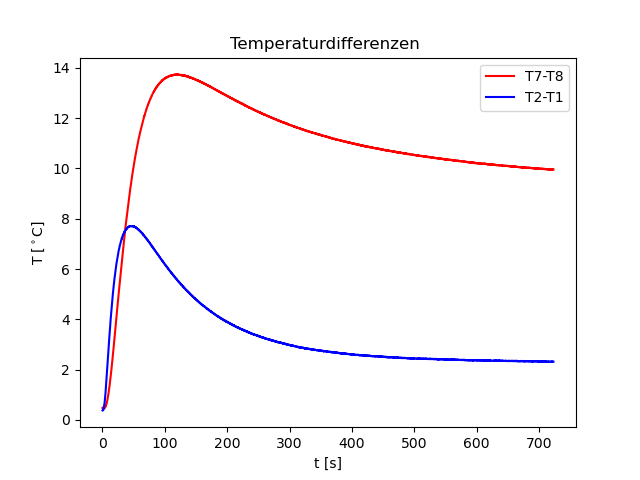
\includegraphics{3.png}
\end{figure}


\subsection{dynamische Methode}

\subsubsection{Bestimmung der Wärmeleitfähigkeit von:}

\subsubsection{Aluminium}

Wenn die Ergebnisse aus der dynamischen Messung für Aluminium graphisch darstellt entsteht folgendes Diagramm:

\begin{figure}[H]
    \centering
    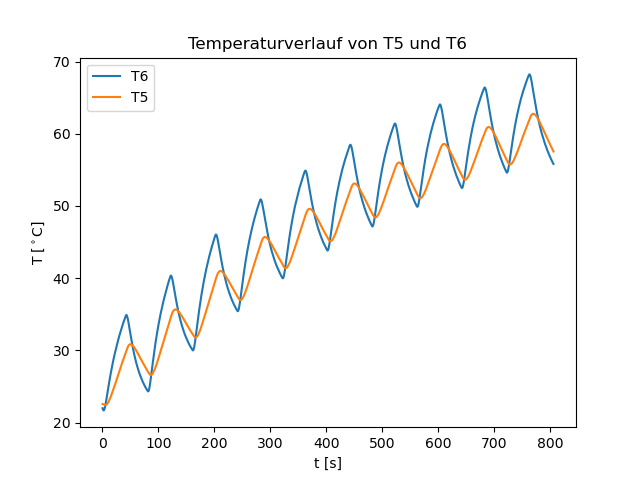
\includegraphics{alu.png}
\end{figure}

Daraus können die Amplituden und die Phasendifferenz der Wellen abgelesen werden. Die abgelesenen Werte sehen wie folgt aus:

\begin{minipage}{\linewidth}
    \begin{table}[H]
        \centering
    \captionof{table}{Amplituden und Phasendifferenz für Aluminium.}
    \begin{tabular}{llll}
        \toprule
        Phasendifferenz & A$_6$ & A$_5$ & $\kappa$  \\
        \midrule
        10 & 34 & 31 & 262.80 \\
        10 & 40 & 35 & 181.80 \\
        10 & 45 & 41 & 260.78 \\
        10 & 51 & 44 & 164.43 \\
        10 & 54 & 49 & 249.84 \\
        10 & 58 & 52 & 222.31 \\
        10 & 61 & 56 & 283.85 \\
        10 & 64 & 58 & 246.60 \\
        10 & 66 & 60 & 254.70 \\
        10 & 68 & 62 & 262.80 \\
        \midrule
        Mittelwerte&für&$\kappa$&238.99$\pm$ 36.27\\
        \bottomrule   
    \end{tabular}
\end{table}
\end{minipage}


\subsubsection{Messing}

Für Messing sieht die Messung folgendermaßen aus:

\begin{figure}[H]
    \centering
    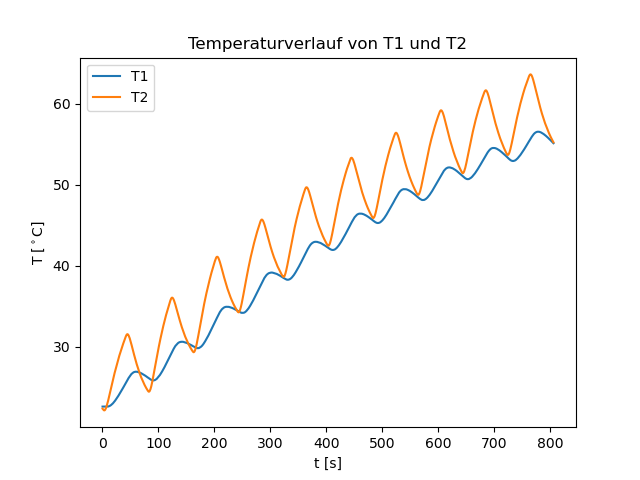
\includegraphics{brass.png}
\end{figure}

\begin{minipage}{\linewidth}
    \begin{table}[H]
        \centering
    \captionof{table}{Amplituden und Phasendifferenz für Aluminium.}
    \begin{tabular}{llll}
        \toprule
        Phasendifferenz & A$_6$ & A$_5$ & $\kappa$  \\
        \midrule
        10 & 32 & 27 & 142.88 \\
        10 & 35 & 31 & 200.03 \\
        10 & 41 & 35 & 153.43 \\
        10 & 45 & 39 & 169.64 \\
        10 & 50 & 43 & 160.96 \\
        10 & 53 & 45 & 148.36 \\
        10 & 55 & 48 & 178.32 \\
        10 & 58 & 50 & 163.56 \\
        10 & 60 & 53 & 195.70 \\
        10 & 62 & 55 & 202.63 \\
        \midrule
        Mittelwerte&für&$\kappa$&171.51$\pm$ 20.67\\
        \bottomrule   
    \end{tabular}
\end{table}
\end{minipage}



\subsubsection{Edelstahl}

Für Edelstahl wurde die 